\section{Looking for communities with Markov Clustering}
\label{mcl}

%% todo: ref to article?

\subsection{Convergency loop}
This loop is repeated a number of times, until the convergence is reached or the maximum
number of loops is executed.
The convergency loop is composed of 3 phases:
\begin{enumerate}
\item Matrix Multiplication, in which the current stochastic matrix is multiplied by itself
\item Matrix Inflation, an operation used to fasten convergency and whose aim and implementation will be explained in the following
\item Matrix Convergence Checker, used to compare achieved values with the previous ones.
\end{enumerate}

Given the matrix $A$ of step $i$, matrix $A'$ output of step $i+1$ has reached the convergency
if the following holds:
$$
\forall i,j . |A_{i,j} - A'_{i,j}| < \epsilon
$$ 
where $\epsilon$ is a parameter of the computation.
In order to minimize occupied space, to fasten convergency and to avoid pathological
cases to lead to "false convergency" (i.e. if the Markov Chain represented by the
matrix is characterized by periodicity), we decided to avoid matrix power method 
and to make the convergency loop proced as the Fibonacci series, meaning
that at step $i$ the matrix calculated in the loop will be $A^{fib(i)}$.
In the following, we will explain in detail the various phases in this convergency
loop.

\subsection{Matrix multiplication}
The first phase of the loop is \textbf{Matrix Multiplication}. For this part, we followed different
approaches for the implementation as map-reduce computations. While the first two approaches
revealed themselves to be very effective when dealing with dummy data using for the tests,
when real data was fetched both showed significant drawbacks that induced us to search for
a third solution, that is the one actually implemented in the delivered project.

\subsubsection{One step map-reduce}
In the beginning, we started by thinking that a simple approach could be producing all
couples to be multiplied of the two matrices with an appropriate index.\footnote{This algorithm
has been readapted and implemented starting from this website: http://importantfish.com/one-step-matrix-multiplication-with-hadoop/}
In this case, we have two different Map functions for two different files. To implement this in Map-Reduce, we exploited
the MultipleInputs function provided by the framework indicating for the two matrices a different mapper able
to emit different values.
The "first" matrix is fetched to the \texttt{OneStepRowMap} of fig. \ref{fig:onestepMaps} while the second to the \texttt{ColumnMap} of the same figure. In the pseudocode, there's no consideration for cases in which the value is 0, since the
matrix is already memorized neglecting null values.
The output of both mappers is fetched to \texttt{OneStepReduce} of fig. \ref{fig:onestepReduce}.
\begin{figure}
\begin{verbatim}
OneStepRowMap(key, value):
    for k = 1 to N:
        emit((value.row, k), ('A', value.column, value.probability))
OneStepColumnMap(key, value)
    for k = 1 to N:
        emit((k, value.column), ('B', value.row, value.probability))
\end{verbatim}
\caption{RowMap and ColumnMap used in the One-Step matrix multiplication algorithm. N is the size of the matrix, which is assumed to be square.}
\label{fig:onestep}
\end{figure}

\begin{figure}
\begin{verbatim}
OneStepReduce(key, values):
    A[N] = {j: a_ij for (x, j, a_ij) in values if x == A}
    B[N] = {j: b_jk for (x, j, b_jk) in values if x == B}
    result = 0
    for j = 1 to N:
        result += hash_A[j] * hash_B[j]
    emit(key, result)
\end{verbatim}
\caption{OneStepReduce used in the One-Step matrix multiplication algorithm. The key represents a single element in the matrix}
\label{fig:onestepReduce}
\end{figure}
As it is possible to understand very easily, with actual data this kind of implementation could not
work, since for every matrix element $N=10^4$ elements are emitted. Elements
are themselves $10^8$, making the total number of couples emitted by the mapper $10^12$.

Approximating the couple (key, value) with the size of its biggest component-
the double precision floating point probability values taking 128 bits on 64 word
machines - we would have needed a total memory of 128TB, which is much larger than
our enviroment total memory space, making impossible to carry on the computation
for dense matrices.

\subsubsection{Two step map-reduce}
The second approach has been the one of decomposing the computation further, trying to avoid
the explosion of data emitted caused by the algorithm discussed before.
In this approach, we have two map reduce steps.\footnote{Once again, this algorithmhas been readapted and implemented
following the post available at http://importantfish.com/two-step-matrix-multiplication-with-hadoop/}

In the mappers shown in fig. \ref{fig:twoStep1Map} used in the first step - again we distinguished between the two matrices using MultipleInputs - rows and columns values are emitted using their index as key.
In the reducer in fig. \ref{fig:twoStep1Reducer}the values of the row and column received are distinguished using the "A" and "B" flags. Subsequently,
every row value is multiplied for every column value, and this multiplied values are emitted using as key
the position of the value of the output matrix to which they will contribute. %todo: cec improbabol inglisc
\begin{figure}
\begin{verbatim}
TwoStepRowMap(key, value):
    emit(value.row, ("A", value.column, value.probability))

TwoStepColumnMap(key, value):
    emit(value.column, ("B", value.row, value.probability))
\end{verbatim}
\caption{Mappers used in the first phase of the two-step matrix multiplication algorithm.}
\label{fig:twoStep1Map}
\end{figure}
\begin{figure}
\begin{verbatim}
reduce(key, values):
    list_A = {(i, a_ij) for (M, i, a_ij) in values if M == "A"}
    list_B = {(k, b_jk) for (M, k, b_jk) in values if M == "B"}
    for (i, a_ij) in list_A:
        for (k, b_jk) in list_B:
            emit((i, k), a_ij*b_jk)
\end{verbatim}
\caption{Reducer used in the first phase of the two-step matrix multiplication algorithm.}
\label{fig:twoStep1Reducer}
\end{figure}

The second map-reduce phase of this algorithm implements the identity function in the mapper, and sums up all
multiplicated values for a certain value of the final matrix in the reducer shown in fig. \ref{fig:twoStep2Reducer}

\begin{figure}
\begin{verbatim}
reduce(key, values):
    result = 0
    for value in values:
        result += value
    emit(key, result)
\end{verbatim}
\caption{Reducer used in the second phase of the two-step matrix multiplication algorithm, summing up al row-by-column values concurring in its calculation.}
\label{fig:twoStep2Reducer}
\end{figure}
Even though this algorithm is way more optimized with respect to the previous one, since it also avoids to emit intermediate couples for possibly null values, it has reveled to be very slow in practice. This is due, in our opinion, to the need
of writing intermediate data between the two steps of the job in HDFS, which slows down computation significantly.

Also in this case some disk problems could arise, because once again, in the worst case, the intermediate data between the two steps is in general $1/2$ of the one emitted by the mapepr in the previous case, making once again
this algorithm unfeasible for the data we were dealing with.
We will se how we solved this problem, by decomposing in smaller parts the input matrix, in the following part.

\subsubsection{Block-wise}
With this approach, to cope with the problems related to the disk, we divided the matrix into several blocks.
Blocks have been enforced to have always the same size, and the approach discussed below has been used.

Let $\mathbf{A}$ and $\mathbf{B}$ be two NxN matrix, and let $p$ be the number of row/column partitions given
as input parameter, meaning that $p^2$ blocks will be produced for each matrix. As an example, we can decompose
A as follows:
$$
\mathbf{A} =
\begin{bmatrix}
    \mathbf{A_{1,1}} & \mathbf{A_{1,2}} & ... & \mathbf{A_{1,p}} \\
    \mathbf{A_{2,1}} & ... & ... \\
    ... \\
    \mathbf{A_{p,1}} & ... & ... & \mathbf{A_{p,p}}
\end{bmatrix}
$$
Now let both $\mathbf{A}$ and $\mathbf{B}$ be decomposed as explained before, we can calculate a single block $\mathbf{C_{i,j}}$
of the matrix $\mathbf{C} = \mathbf{A} x \mathbf{B}$ as follows:
$$
    \mathbf{C_{i,j}} = \sum_{k=1}^{p} \mathbf{A_{i,k}} \times \mathbf{B_{k, j}}
$$
This approach allows, with a sufficient decomposition, to prevent any problem related to disk usage and, in the meanwhile,
produced with some test matrices a way faster computation in the latest implementation.
In fact, the inner multiplication - to be clear, the one between two blocks in the decomposition of the matrices given
as input of this phase - has been implemented in three different way:
\begin{enumerate}
\item In the first case, we tried the (now promising) one-step matrix multiplication algorithm proposed above. However also in this case the output of the mapper revealed himself as huge, as also for a $1/10$-th partition of the matrix (with 1000 values) this approach would produce $10^9$ values, which is certainly a manageable size but still big enough to slow down the computation significantly, specially when considering the huge number of such multiplications to perform to calculate the whole $\mathbf{C}.$
\item In the second case, to be honest merely for the sake of completeness, we tried also to plug-in as multiplication module the two-step matrix multiplication algorithm. As it could have been foreseen, also this approach - though faster than the previous one - was still not fast enough to meet our requirements.
\item The third case, which is the one used in the final project, revealed himself to be the best both in terms of space and in completion time. This algorithm merely multiplies two blocks using the good old $O(n^3)$ sequential row-by-column matrix multiplication.
\end{enumerate}

As it is possible to understand, the approach that we finally decided to follow is very efficient for several resons.
Consider the case in which the number of partitions is 10, thus achieving 100 blocks for each of the two multiplied matrices.
The blocks will contain, in a worst case approximaton, $10^6$ doubles, meaning that a block multiplication will fit in memory and thus result in better performances, since also the output of each block-by-block multiplication will have size of approximately 32MB each, considering also the indexes.

Notice that this values, on our environment, allow to multiply several blocks in parallel, leading to a very good utilization
factor of the machines and nice results in terms of completion time.
The detailed implementation of this part is discussed thoroughly in \ref{blockmul}.

\subsubsection{Block-wise multiplication implementation}
\label{blockmul}
We wanted to develop, in this part, an highly parametrized system so to finely tune our computation to make it faster,
given that this is the biggest contributor to the completion time of the convergency loop, which is executed also several times.
For this reason, a module, called BlockWiseMatrixMultiplication has been developed, with the aim of allowing parametrized execution.

This module, which implements the \texttt{Tool} interface of the Hadoop framework, can be executed specifying the number
of blocks of the final matrix $\mathbf{C_{i,j}}$ to be executed in parallel. It takes also in input the directory containing
the two input matrices splitted in blocks and the directory in which the results must be written. Partitions are 
calculated automatically scanning the blocks by horizontal coordinates (by row) and then by column.

For each block multiplication scheduled by this very simple partitioner, a new thread is forked, which is responsible
for starting and monitoring all the jobs (running in parallel) consisting of the multiplications $\mathbf{A_{i,k}} \times \mathbf{B_{k,j}}$ needed to calculate $\mathbf{C_{i,j}}$.

In order for them to run in parallel, we used the \texttt{JobControl} class of the Hadoop framework, which allows to
schedule parallel jobs (and also to define dependencies between jobs). For every output block $\mathbf{C_{i,j}}$ $p$ 
multiplications of the original matrix blocks are performed as independent jobs running in parallel. 
These jobs consist of a single map-reduce phase, in which the mappers (as usual, one for the row and one for the column exploiting MultipleInputs) of fig. \ref{fig:blockwisemap} take care of "joining" and labelling the two blocks to be multiplied.
In the reducer, the whole blocks are gathered and saved in a matrix, which is then multiplied before the final values
are written in output, as it is possible to see in fig. \ref{fig:blockwisereduce}.
In the reducer, a slight optimization has been achieved by memorizing the second matrix (accessed k times) by column
and not by row, to avoid jumps in memory and to exploit caches and memory in the best possible way.

\begin{figure}
\begin{verbatim}
BlockRowMapper(key, value):
    emit(value.blockVerticalIndex, ('A', value.row_id, value.column_id, value.probability))


BlockColumnMapper(key, value):
    emit(value.blockHorizontalIndex, ('B', value.row_id, value.column_id, value.probability))
\end{verbatim}
\caption{Mappers used in the block-wise matrix multiplication. The block $\mathbf{A_{i,k}}$ is managed by BlockRowMapper, while $\mathbf{B_{k,j}}$ by BlockColumnMapper. This names are given merely for consinstency wrt. previous algorithms} 
\label{fig:blockwisemap}
\end{figure}

\begin{figure}
\begin{verbatim}
MatrixMultiplicationReducer(key, values):
    A[N/p][N/p]
    B[N/p][N/p]
    for v in values
        if v.label = 'A'
            A[v.row_id][v.col_id] = v.probability
        else
            B[v.col_id][v.row_id] = v.probability
    for i in [1, N/p]
        for j in [1, N/p]
            sum = 0
            for k in [1, N/p]
                sum += A[i][k]*B[j][k]
            if sum > 0
                emit((i,j), sum)
\end{verbatim}
\caption{Reducer used in the block-wise matrix multiplication. It performs the usual row-by-column matrix multiplication algorithm. N is the size of the matrix, p is the number of splits}
\label{fig:blockwisereduce}
\end{figure}
The second job needed to finally compute $\mathbf{C_{i,j}}$ is the one performing the sum over all partial matrices produced before, in order to achieve the real values in the computed block.
This job has, in its configuration, the horizontal and vertical coordinates $i$ and $j$ of the output block. In its mapper of fig. \ref{fig:blocksummap}, it aggregates by block row id and block column id the elements, so that they can be subsequently summed in the reducer as of fig. \ref{fig:blocksumreduce}.
This job is dependant of the previous ones, thus starts as soon as all the input data needed has been produced.
\begin{figure}
\begin{verbatim}
BlockSumMapper(key, value):
    emit((value.row_id, value.col_id), value.probability)
\end{verbatim}
\caption{The map function used to perform the sum over all partial matrices $\mathbf{A_{i,k}} \times \mathbf{B_{k,j}}$ and thus to calculate $\mathbf{C_{i,j}}$}
\label{fig:blocksummap}
\end{figure}
\begin{figure}
\begin{verbatim}
BlockSumReducer(key, values):
    blockIdX = get(block.horizontal_coordinates)
    blockIdY = get(block.vertical_coordinates)
    sum = 0
    for v in values
        sum += v
    emit((blockIdX, blockIdY, key.row_id, key._column_id), sum)
\end{verbatim}
\caption{The reduce function used to calculate the sum over single values in a position of the block and which writes out the final block.}
\label{fig:blocksumreduce}
\end{figure}
The thread forked and running the JobControl containing all such "individual block" jobs running in parallel, is checked periodically by another thread for completion. When this phase terminates, another set of blocks of parametric size
is calculated and the related multiplications are run.
This approach of not running everything in parallel has been pursued in order to avoid disk space issues and also to be 
able to avoid too much contention in the system.
From experimental results, in fact, we were able to verify that the matrix multiplication can be made very fast by dividing
initial matrices in 25 blocks and using partitions of size from 5 (corresponding thus to an entire row).

The drawback of this approach is that some others modules - for decomposing and recomposing the matrix - must be executed, as we wanted our procedure not to affect the final matrix representation.

These modules implementation is discussed in \ref{splitter} and \ref{recombiner}.
Finally, the behaviour of a single block multiplication is sketched in fig. \ref{fig:blockmultiplicationsketch}, while
the comprehensive driver of the matrix multiplication procedure that we finally adopted is illustrated in fig. \ref{fig:matrixmultiplicationsketch}, and its source code can be seen on %todo: insert link.

\begin{figure}
\centering
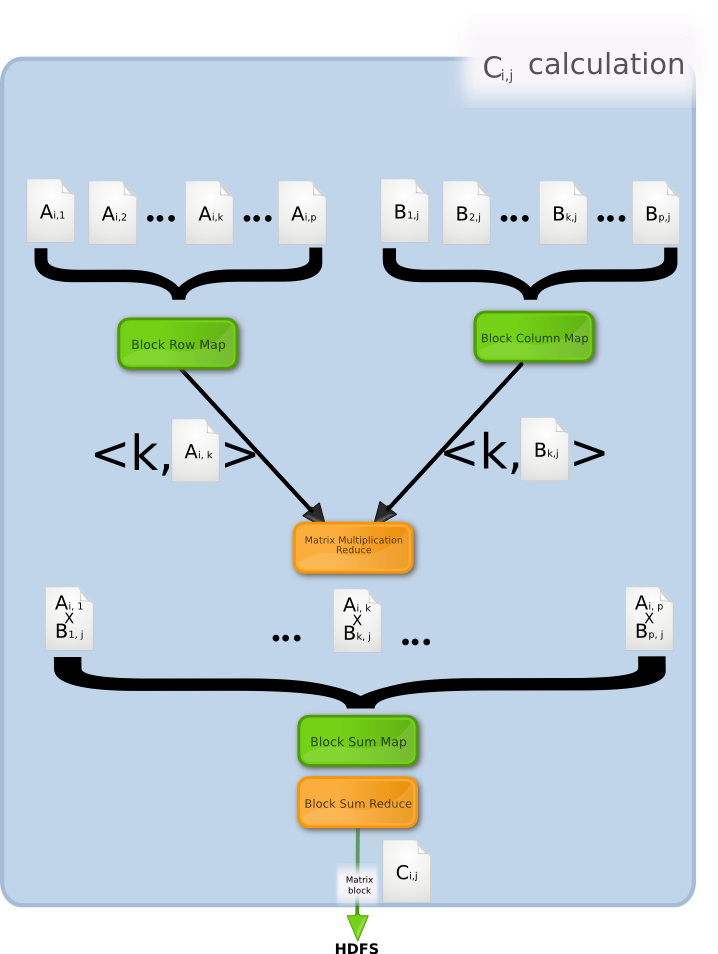
\includegraphics[scale=0.7]{blockmultiplication.png}
\caption{Procedure followed to calculate a single $\mathbf{C_{i,j}}$.}
\label{fig:blockmultiplicationsketch}
\end{figure}

\begin{figure}
\centering
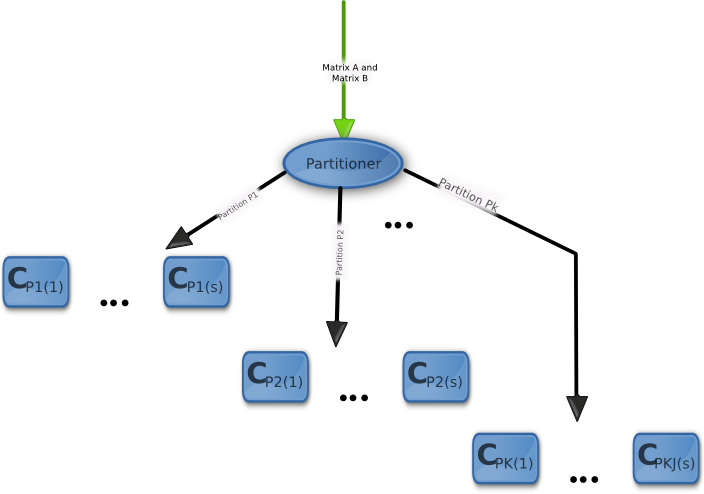
\includegraphics[scale=0.7]{matrixmultiplication.png}
\caption{Whole matrix multiplication procedure in a block-wise fashion. S blocks of the matrix are calculated
in parallel, while the others wait for the completion of the previous ones before going on.
In the image, s is the maximum size of the partition, k is assumed as the number of partitions and Pi(n) is a function
returning the index of the n-th block in partition Pi.In the image, the blue blocks titled after the matrix block they are used to compute represent the calculation shown in fig. \ref{fig:blockmultiplicationsketch}}
\label{fig:matrixmultiplicationsketch}
\end{figure}

\subsection{Inflation}

After multiplying the matrix by the last precedently computed, we apply a strategy
called inflation in order to enlarge differences between elements in a row.

For each row, we compute the sum of all r-th powers of its elements.
Then we recompute the element i,j as
$$ a_{i,j} = \frac{a_{ij}^r} {\sum_{k=0..N} a_{ik}^r}$$


\subsection{Convergency}

Actually, 


\subsection{Matrix splitter}
\label{splitter}
\subsection{Matrix recombiner}
\label{recombiner}
\subsection{Driver}